\newif\ifuseOldExample
% uncomment the following to use the old DemonstratingExample
\useOldExampletrue

\chapter{\Compose*{}}
\begin{flushright}
\textit{``The difficult part of composition filters}\\
\textit{is understanding its simplicity.''}\\
\textit{Lodewijk Bergmans}\\
\end{flushright}

\label{chp:ComposeStar}

\Compose* is an implementation of the composition filters approach. There are three target environments: the \dotNET, Java, and C.
This chapter is organized as follows, first the evolution of Composition Filters and its implementations are described, followed by an explanation of the \Compose* language and a demonstrating example. 
In the third section, the \Compose* architecture is explained, followed by a description of the features specific to \Compose*.

\section{Evolution of Composition Filters}
\Compose* is the result of many years of research and experimentation.
The following time line gives an overview of what has been done in the years before and during the \Compose* project.

\begin{description}[noitemsep,style=sameline,leftmargin=15mm]
\item[1985] The first version of Sina is developed by Mehmet Ak\c{s}it.
            This version of Sina contains a preliminary version of the composition filters concept called semantic networks.
            The semantic network construction serves as an extension to objects, such as classes, messages, or instances.
            These objects can be configured to form other objects such as classes from which instances can be created.
            The object manager takes care of synchronization and message processing of an object.
            The semantic network construction can express key concepts like delegation, reflection, and synchronization~\cite{koopmans:sina95}.
\item[1987] Together with Anand Tripathi of the University of Minnesota the Sina language is further developed.
            The semantic network approach is replaced by declarative specifications and the interface predicate construct is added.
\item[1991] The interface predicates are replaced by the dispatch filter, and the wait filter manages the synchronization functions of the object manager.
            Message reflection and real-time specifications are handled by the meta filter and the real-time filter~\cite{bergmans:phd94}.
\item[1995] The Sina language with Composition Filters is implemented using Smalltalk~\cite{koopmans:sina95}.
            The implementation supports most of the filter types.
            In the same year, a preprocessor providing C++ with support for Composition Filters is implemented~\cite{glandrup:ms95}.
\item[1999] The composition filters language ComposeJ~\cite{wichman:ms99} is developed and implemented.
            The implementation consists of a preprocessor capable of translating composition filter specifications into the Java language.
\item[2001] ConcernJ is implemented as part of a \MSc thesis~\cite{salinas:ms01}.
            ConcernJ adds the notion of superimposition to Composition Filters.
            This allows for reuse of the filter modules and to facilitate crosscutting concerns.
\item[2003] The start of the \Compose* project, the project is described in further detail in this chapter.
\item[2004] The first release of \Compose*, based on \dotNET.
\item[2005] The start of the Java port of \Compose*.
\item[2006] Porting \Compose* to C is started.
\end{description}

%\section{Composition Filters}
\section{Composition Filters in \Compose*{}}
\label{sec:CompositionFiltersInComposeStar}
% Removed "t" so that it is not longer breaking the history list
\begin{lstlisting}[language=Composestar,style=floatlisting,float=hbp, caption={Abstract concern template},label={lst:concerntemplate}]
concern {
  filtermodule {
    internals
    externals
    conditions
    inputfilters
    outputfilters
  }
  superimposition {
    selectors
    filtermodules
    annotations
    constraints
  }
  implementation
}
\end{lstlisting}
A \Compose* application consists of concerns that can be divided in three parts: filter module specifications, superimposition, and implementation.
A filter module contains the filter logic to filter on incoming or outgoing messages on superimposed objects.
Messages have a target, which is an object reference, and a selector, which is a method name.
A superimposition part specifies which filter modules, annotations, conditions, and methods are superimposed on which objects.
An implementation part contains the class implementation of a concern.
How these parts are placed in a concern is shown in \autoref{lst:concerntemplate}.

\begin{figure}[hbp]
  \centering
  \includegraphics[style=thirdheight]{cfmodel}
  \caption{Components of the composition filters model}
  \label{fig:cfmodel}
\end{figure}

The working of a filter module is depicted in \autoref{fig:cfmodel}.
A filter module can contain input and output filters.
The difference between these two sets of filters is that the first is used to filter on incoming messages, while the second is used to filter on outgoing messages.
The return of a method is not considered an outgoing message.
A filter has three parts: a filter identifier, a filter type, and one or more filter elements.
A filter element exists out of an optional condition part, a matching part, and a substitution part.
These parts are shown below:
\begin{center}
$\overbrace{stalker\_filter}^{identifier}:\overbrace{Dispatch}^{filter~type}~=~\{\overbrace{!pacmanIsEvil}^{condition~part}
=>\overbrace{[*.getNextMove]}^{matching~part}~\overbrace{stalk\_strategy.getNextMove}^{substitution~part}~\}$
\end{center}
A filter identifier is a unique name for a filter in a filter module. 
Filters match when both the condition part and the matching part evaluate to true.
In the demonstrated filter, every message where the selector is \lstinline|getNextMove| matches.
If an asterisk~(\lstinline|*|) is used in the target, every target will match.
When the condition part and the matching part are true, the message is substituted with the values provided in the substitution part.
How these values are substituted, and how the message continues, depends on the type of  filter used.
\newpage
At the moment there are four basic filter types defined in \Compose*.
It is, however, possible to write custom filter types.
\begin{description}[style=sameline,leftmargin=18mm]
  \item[Dispatch] If the message is accepted, it is dispatched to the specified target of the message, otherwise the message continues to the subsequent filter.
    This filter type can only be used for input filters;
  \item[Send] If the message is accepted, it is sent to the specified target of the message, otherwise the message continues to the subsequent filter.
    This filter type can only be used for output filters;
  \item[Error] If the filter rejects the message, it raises an exception, otherwise the message continues to the next filter in the set;
  \item[Meta] If the message is accepted, the message is sent as a parameter of another meta message to an internal or external object, otherwise the message just continues to the next filter.
    The object that receives the meta message can observe and manipulate the message and can re-activate the execution of the message.
\end{description}

The identifier \lstinline|pacmanIsEvil|, used in the condition part, must be declared in the conditions section of a filter module.
Targets that are used in a filter can be declared as internal or external.
An internal is an object that is unique for each instance of a filter module, while an external is an object that is shared between filter modules.

Filter modules are superimposed on classes using filter module binding, which specifies a selection of objects on the one side, and a filter module on the other side.
The selection is specified in a selector definition.
This selector definition uses predicates to select objects, such as \lstinline|isClassWithNameInList|, \hbox{\lstinline|isNamespaceWithName|}, and \lstinline|namespaceHasClass|.
In addition to filter modules, it is possible to bind conditions, methods, and annotations to classes using superimposition.

The last part of the concern is the implementation part, which can be used to define the behavior of a concern.
For a logging concern, for example, we can define specific log functions and use them as internal.



%\section{Demonstrating Example}
\ifuseOldExample
	% Pacman 1 example
	\section{Demonstrating Example}
\label{sec:demonstratingexample}

To illustrate the \Compose* toolset, this section introduces a \emph{Pacman} example.
The Pacman game is a classic arcade game in which the user, represented by pacman, moves in a maze to eat vitamins.
Meanwhile, a number of ghosts try to catch and eat pacman.
There are, however, four mega vitamins in the maze that make pacman evil.
In its evil state, pacman can eat ghosts.
A simple list of requirements for the Pacman game is briefly discussed here:
\begin{itemize}[noitemsep]
  \item One live is taken from pacman when eaten by a ghost;
  \item A game should end when pacman has no more lives;
  \item The score of a game should increase when pacman eats a vitamin or a ghost;
  \item A user should be able to use a keyboard to move pacman around the maze;
  \item Ghosts should know whether pacman is evil or not;
  \item Ghosts should know where pacman is located;
  \item Ghosts should hunt or flee from pacman, depending on the state of pacman.
\end{itemize}

\subsection{Initial Object-Oriented Design}

\begin{figure}[p]
  \centering
  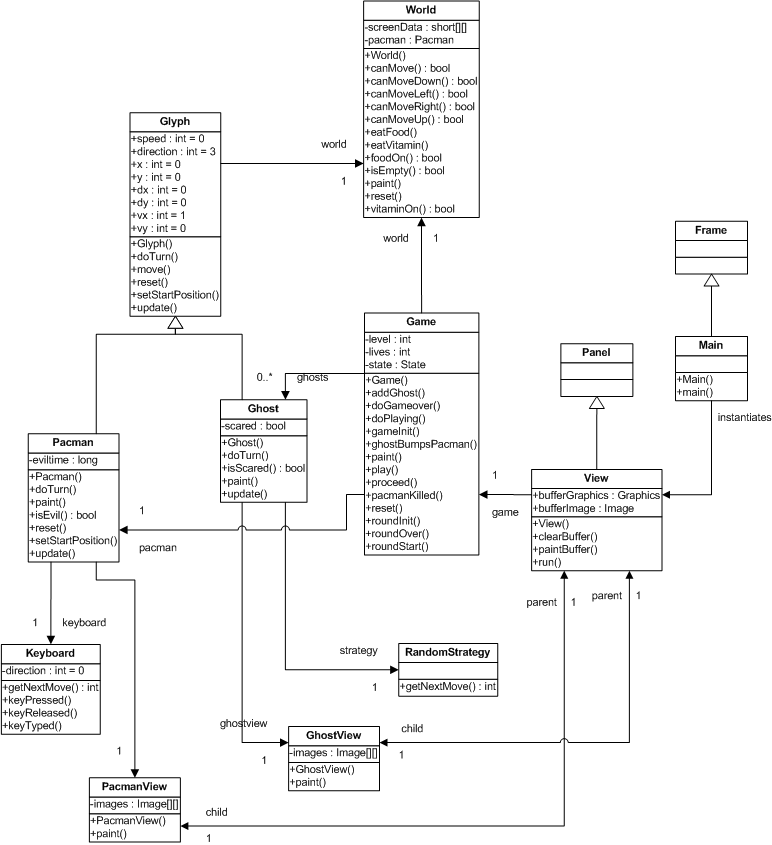
\includegraphics[style=page]{pacman_class_diagram}
  \caption{Class diagram of the object-oriented Pacman game}
  \label{fig:pacman_class_diagram}
\end{figure}
\afterpage{\clearpage}

\nomenclature{UML}{Unified Modeling Language}%
\autoref{fig:pacman_class_diagram} shows an initial object-oriented design for the Pacman game.
Note that this UML class diagram does not show the trivial accessors.
The classes in this diagram are:
%\begin{description}[noitemsep,style=nextline]
\begin{description}[noitemsep,style=sameline,leftmargin=32mm]
  \item [Game] This class encapsulates the control flow and controls the state of a game;
  \item [Ghost] This class is a representation of a ghost chasing pacman.
    Its main attribute is a property that indicates whether it is scared or not (depending on the evil state of pacman);
  \item [GhostView] This class is responsible for painting ghosts;
  \item [Glyph] This is the superclass of all mobile objects (pacman and ghosts).
    It contains common information like direction and speed;
  \item [Keyboard] This class accepts all keyboard input and makes it available to pacman;
  \item [Main] This is the entry point of a game;
  \item [Pacman] This is a representation of the user controlled element in the game.
    Its main attribute is a property that indicates whether pacman is evil or not;
  \item [PacmanView] This class is responsible for painting pacman;
  \item [RandomStrategy] By using this strategy, ghosts move in random directions;
  \item [View] This class is responsible for painting a maze;
  \item [World] This class has all the information about a maze.
    It knows where the vitamins, mega vitamins and most importantly the walls are.
    Every class derived from class \lstinline|Glyph| checks whether movement in the desired direction is possible.
\end{description}

\subsection{Completing the Pacman Example}

The initial object-oriented design, described in the previous section, does not implement all the stated system requirements.
The missing requirements are:
\begin{itemize}[noitemsep]
  \samepage
  \item The application does not maintain a score for the user;
  \item Ghosts move in random directions instead of chasing or fleeing from pacman.
\end{itemize}
In the next sections, we describe why and how to implement these requirements in the \Compose* language.

\subsubsection{Implementation of Scoring}

The first system requirement that we need to add to the existing Pacman game is scoring.
This concern involves a number of events.
First, the score should be set to zero when a game starts.
Second, the score should be updated whenever pacman eats a vitamin, mega vitamin or ghost.
And finally, the score itself has to be painted on the maze canvas to relay it back to the user.
These events scatter over multiple classes: \lstinline|Game| (initializing score), \lstinline|World| (updating score), \lstinline|Main| (painting score).
Thus scoring is an example of a crosscutting concern. 

To implement scoring in the \Compose* language, we divide the implementation into two parts.
The first part is a \Compose* concern definition stating which filter modules to superimpose.
\autoref{lst:scoringconcern} shows an example \Compose* concern definition of scoring.

\begin{lstlisting}[style=listing,escapeinside={&$}{$&},language=ComposeStar,%
                   caption={\expandafter{\lstinline[style=inline]|DynamicScoring|} concern in \Compose*{}},%
                   label={lst:scoringconcern}]
concern DynamicScoring in Pacman {&$\label{line:dynscore_concern}$&
  filtermodule dynamicscoring {&$\label{line:dynscore_fm_begin}$&
    externals
      score : pacman.Score = pacman.Score.instance();
    inputfilters 
      score_filter : Meta = {[*.eatFood] score.eatFood,&$\label{line:score_filter}$&
                             [*.eatGhost] score.eatGhost,
                             [*.eatVitamin] score.eatVitamin,
                             [*.gameInit] score.initScore,
                             [*.setForeground] score.setupLabel}
  }&$\label{line:dynscore_fm_end}$&
  superimposition {&$\label{line:dynscore_si_begin}$&
    selectors
      scoring = { C | isClassWithNameInList(C, ['pacman.World',
                                 'pacman.Game', 'pacman.Main']) };
    filtermodules
      scoring <- dynamicscoring;
  }&$\label{line:dynscore_si_end}$&
}
\end{lstlisting}

This concern definition is called \lstinline|DynamicScoring| (line~\ref{line:dynscore_concern}) and contains two parts.
The first part is the declaration of a filter module called \lstinline|dynamicscoring| (lines~\ref{line:dynscore_fm_begin}--\ref{line:dynscore_fm_end}).
This filter module contains one \emph{meta filter} called \lstinline|score_filter| (line~\ref{line:score_filter}).
This filter intercepts five relevant calls and sends the message in a reified form to an instance of class \lstinline|Score|.
The final part of the concern definition is the superimposition part (lines~\ref{line:dynscore_si_begin}--\ref{line:dynscore_si_end}).
This part defines that the filter module \lstinline|dynamicscoring| is to be superimposed on the classes \lstinline|World|, \lstinline|Game| and \lstinline|Main|.

The final part of the scoring concern is the so-called \emph{implementation part}.
This part is defined by a class \lstinline|Score|.
\autoref{lst:scoreimpl} shows an example implementation of class \lstinline|Score|.
Instances of this class receive the messages sent by \lstinline|score_filter| and subsequently perform the events related to the scoring concern.
In this way, all scoring events are encapsulated in one class and one \Compose* concern definition. 

\begin{lstlisting}[style=floatlisting,language=Java,%
                   caption={Implementation of class \expandafter{\lstinline[style=inline]|Score|}},%
                   label={lst:scoreimpl}]
public class Score 
{
  private int score = -100;
  private static Score theScore = null;
  private Label label = new java.awt.Label("Score: 0");

  private Score() {}

  public static Score instance() {
    if(theScore == null) {
      theScore = new Score();
    }
    return theScore;
  }

  public void initScore(ReifiedMessage rm) {
    this.score = 0;
    label.setText("Score: "+score);
  }

  public void eatGhost(ReifiedMessage rm) {
    score += 25;
    label.setText("Score: "+score);
  }

  public void eatVitamin(ReifiedMessage rm) {
    score += 15;
    label.setText("Score: "+score);
  }

  public void eatFood(ReifiedMessage rm) {
    score += 5;
    label.setText("Score: "+score);
  }

  public void setupLabel(ReifiedMessage rm) {
    rm.proceed();
    label = new Label("Score: 0");
    label.setSize(15*View.BLOCKSIZE+20,15*View.BLOCKSIZE);
    Main main = (Main)Composestar.Runtime.FLIRT.message.MessageInfo.getMessageInfo().getTarget();
    main.add(label,BorderLayout.SOUTH);
  }
}
\end{lstlisting}

\subsubsection{Implementation of Dynamic Strategy}

The last system requirement that we need to implement is the dynamic strategy of ghosts.
This means that a ghost should, depending on the state of pacman, hunt or flee from pacman.
We can implement this concern by using the strategy design pattern.
However, in this way, we need to modify the existing code.
This is not the case when we use \Compose*{} \emph{dispatch filters}.
\autoref{lst:dynamicstrategyconcern} demonstrates this. 

\begin{lstlisting}[style=floatlisting,escapeinside={&$}{$&},language=Composestar,%
                   xrightmargin=-25mm,%
                   caption={\expandafter{\lstinline[style=inline]|DynamicStrategy|} concern in \Compose*{}},%
                   label={lst:dynamicstrategyconcern}]
concern DynamicStrategy in Pacman {
  filtermodule dynamicstrategy {
    internals
      stalk_strategy : pacman.Strategies.StalkerStrategy;
      flee_strategy : pacman.Strategies.FleeStrategy;   
    conditions
      pacmanIsEvil : pacman.Pacman.isEvil();
    inputfilters
      stalker_filter : Dispatch = {!pacmanIsEvil =>&$\label{line:stalker_filter}$&
                        [*.getNextMove] stalk_strategy.getNextMove};
      flee_filter : Dispatch = {&$\label{line:flee_filter}$&
                        [*.getNextMove] flee_strategy.getNextMove}
  }
  superimposition {
    selectors
      random = { C | isClassWithName(C,
                        'pacman.Strategies.RandomStrategy') };
    filtermodules
      random <- dynamicstrategy;
  }
}
\end{lstlisting}

This concern uses dispatch filters to intercept calls to method \lstinline|getNextMove| of the class \lstinline|RandomStrategy|.
These calls are redirected to either \lstinline|StalkerStrategy.getNextMove| or \lstinline|FleeStrategy.getNextMove|.
If pacman is not evil, the intercepted call matches the first filter, which dispatches the intercepted call to method \lstinline|StalkerStrategy.getNextMove| (line~\ref{line:stalker_filter}).
Otherwise, the intercepted call matches the second filter, which dispatches the intercepted call to method \lstinline|FleeStrategy.getNextMove| (line~\ref{line:flee_filter}).


\else	
	% Pacman 2 example (used as of April 2007)
	\newpage
\section{Demonstrating Example}
\label{sec:demonstratingexample}

To illustrate the \Compose* toolset, this section introduces a \emph{Pac-Man} example.
The Pac-Man game is a classic arcade game in which the user, represented by Pac-Man, moves in a maze to eat pills.
Meanwhile, a number of ghosts try to catch and eat Pac-Man.
There are, however, four power pills in the maze that make Pac-Man evil. In its evil state, Pac-Man can eat ghosts.

A simple list of requirements for the Pac-Man game is briefly discussed here:
\begin{itemize}[noitemsep]
  \item The number of lives taken from Pac-Man when eaten by a ghost;
  \item A game should end when Pac-Man has no more lives;
  \item The score of a game should increase when Pac-Man eats a pill or a ghost;
  \item A user should be able to use a keyboard to move Pac-Man around the maze;
  \item Ghosts should know whether Pac-Man is evil or not;
  \item Ghosts should know where Pac-Man is located;
  \item Ghosts should, depending on the state of Pac-Man, hunt or flee from Pac-Man;
  \item At fixed intervals a bonus item should appear that gives bonus points when eaten by Pac-Man.
\end{itemize}

\subsection{Initial Object-Oriented Design}

\begin{figure}[p]
  \centering
  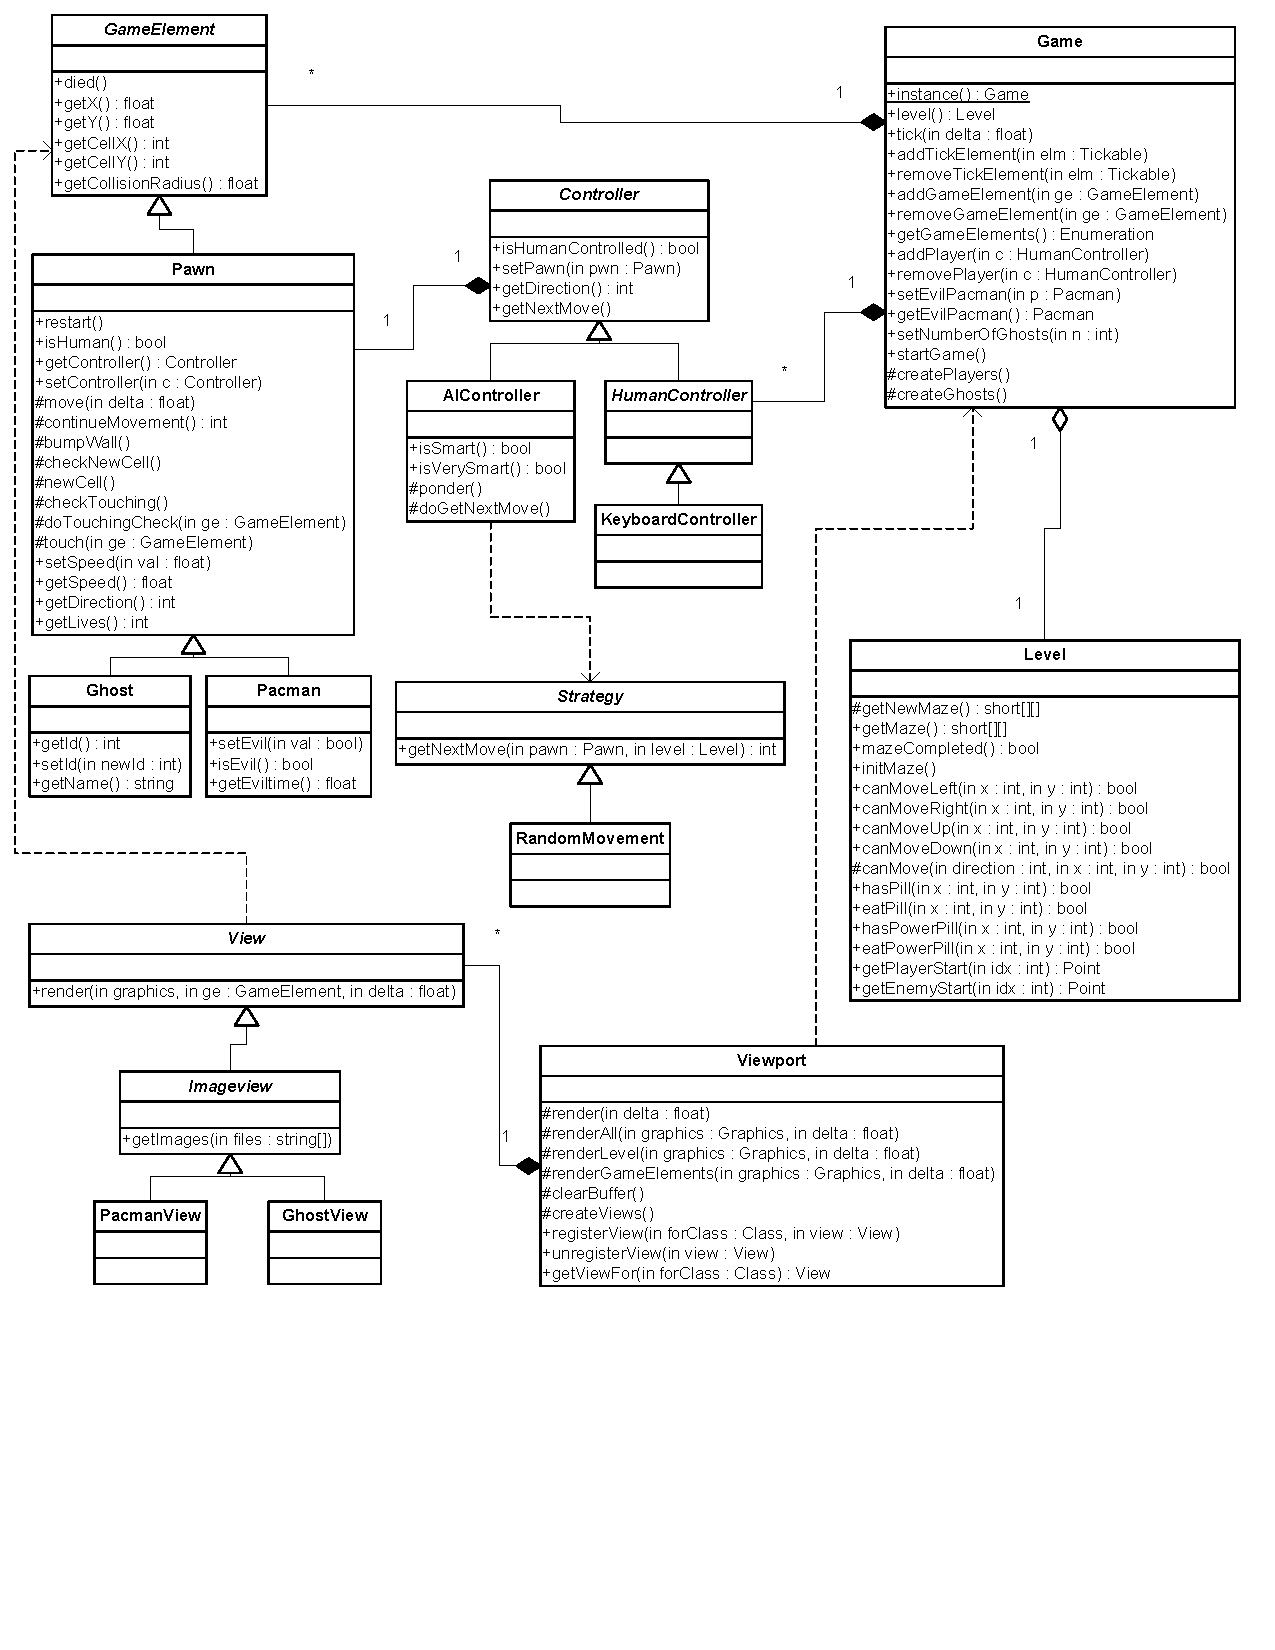
\includegraphics[style=page]{PacmanTwo}
  \caption{Class diagram of the object-oriented Pac-Man game}
  \label{fig:pacman2_class_diagram}
\end{figure}

\nomenclature{UML}{Unified Modeling Language}%
\autoref{fig:pacman2_class_diagram} shows an initial object-oriented design for the Pac-Man game.
Note that this UML class diagram does not show the class attributes.
The classes in this diagram are:
\begin{description}[noitemsep,style=sameline,leftmargin=32mm]
	\item[AIController] The \lstinline|AIController| is used for the non user controlled pawns. It makes 
		use of a \lstinline|Strategy| class	to determine the next move;
	\item[Controller] The controller is responsible for providing the \lstinline|Pawn| with the desired 
		direction of movement. A controller is either user controller or computer controlled;
	\item[Game] This class encapsulates the control flow and controls the state of a game;
	\item[GameElement] This is the base class for all, with the exception of the pills, visual elements 
		in the game. A \lstinline|GameElement| has a position within the maze and a collision radius;
	\item[Ghost] This class is a representation of a ghost chasing Pac-Man. Each ghost has an identifier
	  that can be used to change the behavior for individual ghosts;	
	\item[HumanController] The \lstinline|HumanController| is an abstract controller class that receives movement 
		instructions from a user;
	\item[KeyboardController] The \lstinline|KeyboardController| is an implementation of the \lstinline|HumanController|
	  that reads the instructions from the keyboard;			
	\item[Level] This class contains the structural information of the maze, this includes information about the walls,
		location of the pills, and starting locations of Pac-Man and the ghosts. It contains methods to check for, and eat
		the pills in the maze. It also has method to check for walls in a given direction;
	\item[Pacman] This is a representation of the user controlled pawn in the game. It contains a flag that tells if
		the Pac-Man is in evil mode;
	\item[Pawn] The \lstinline|Pawn| class is used for all non stationary \lstinline|GameElement|s. Pawns are 
		controlled by an instance of the \lstinline|Controller| class. It has a speed, direction and number of lives.
		The pawn performs collision checks after every move and acts accordingly. A pawn will continue moving in the
		set direction with the given speed until these parameters have been changed;
	\item[RandomMovement] The \lstinline|RandomMovement| class returns a random direction the given pawn can move to;
	\item[Strategy] This class is used by the \lstinline|AIController| to make a movement choice;
	\item[View] \lstinline|GameElement|s are drawn on the \lstinline|Viewport| using a \lstinline|View| implementation 
		that has been registered with the \lstinline|Viewport|.	Each \lstinline|GameElement| implementation has	its own 
		\lstinline|View| subclass;
	\item[Viewport] The \lstinline|Viewport| shows the current game to the player. It is responsible for rendering 
		the maze and delegates rendering of the \lstinline|GameElement|s to the associated \lstinline|View| instances.
\end{description}

\subsection{Completing the Pac-Man Example}

The initial object-oriented design, described in the previous section, does not implement all the stated system requirements.
The missing requirements are:
\begin{itemize}[noitemsep]
  \samepage
  \item The application does not maintain a score for the user;
  \item Ghosts move in random directions instead of chasing or fleeing from Pac-Man;
  \item There is no bonus item that Pac-Man can pick up.
\end{itemize}
In the next sections, we describe why and how to implement these requirements in the \Compose* language.

\subsubsection{Implementation of Scoring}
\label{sec:scoring_concern}

The first system requirement that we need to add to the existing Pac-Man game is scoring.
This concern involves a number of events.
The score should be updated whenever Pac-Man eats a pill, power pill or ghost.
And the score itself has to be drawn on the screen to relay it back to the user.
These events scatter over multiple classes: \lstinline|Level| (updating score), \lstinline|Ghost| (updating score), \lstinline|Viewport| (drawning score).
Thus scoring is an example of a crosscutting concern where only new behavior is added without changing the original behavior of the program.

To implement scoring in the \Compose* language, we divide the implementation into two parts.
The first part is a \Compose* concern definition stating which filter modules to superimpose.
\autoref{lst:scoringconcern} shows an example \Compose* concern definition of scoring.

\begin{lstlisting}[style=floatlisting,escapeinside={&$}{$&},language=ComposeStar,%
                   caption={\expandafter{\lstinline[style=inline]|Scoring|} concern in \Compose*{}},%
                   label={lst:scoringconcern}]
concern Scoring in PacmanTwo&$\label{line:scoring_concern}$&
{
	filtermodule registerScorePawns&$\label{line:scoring_fm_rsp}$&
	{
		externals
			score : PacmanTwo.Scoring.Score = PacmanTwo.Scoring.Score.instance();
		inputfilters
			scored : After = { [*.died] score.pawnDied }&$\label{line:scoring_fm_rsp_scored}$&
	}&$\label{line:scoring_fm_rsp_end}$&

	filtermodule registerScoreLevel&$\label{line:scoring_fm_rsl}$&
	{
		externals
			score : PacmanTwo.Scoring.Score = PacmanTwo.Scoring.Score.instance();
		inputfilters
			scored : After = { [*.eatPill] score.eatPill
			                 , [*.eatPowerPill] score.eatPowerPill }
	}&$\label{line:scoring_fm_rsl_end}$&

	filtermodule renderScore&$\label{line:scoring_fm_rs}$&
	{
		internals
			scoreview : PacmanTwo.Scoring.ScoreView;
		inputfilters
			render : After = { [*.renderAll] scoreview.renderScore }
	}&$\label{line:scoring_fm_rs_end}$&

	superimposition&$\label{line:scoring_si}$&
	{
		selectors
			lvl = { C | isClassWithName(C, 'PacmanTwo.Level') };
			pawns = { C | isClassWithNameInList(C, ['PacmanTwo.Ghost']) };
			viewport = { C | isClassWithName(C, 'PacmanTwo.GUI.Viewport' ) };
		filtermodules
			lvl <- registerScoreLevel;
			pawns <- registerScorePawns;
			viewport <- renderScore;
	}&$\label{line:scoring_si_end}$&
}
\end{lstlisting}

This concern definition is called \lstinline|Scoring| (line~\ref{line:scoring_concern}) and contains two parts.
The first part is the declaration of the filter modules called \lstinline|registerScorePawns| (lines~\ref{line:scoring_fm_rsp}--\ref{line:scoring_fm_rsp_end}), \lstinline|registerScoreLevel| (lines~\ref{line:scoring_fm_rsl}--\ref{line:scoring_fm_rsl_end}), and \lstinline|renderScore| (lines~\ref{line:scoring_fm_rs}--\ref{line:scoring_fm_rs_end}).
The first two filter modules \lstinline|registerScorePawns| and \lstinline|registerScoreLevel| will update the current score. When Pac-Man eats a ghost the \lstinline|died| method will be called on the \lstinline|Ghost|. 
The filter module \lstinline|registerScorePawns| contains an \emph{after filter} called \lstinline|scored| (line~\ref{line:scoring_fm_rsp_scored}). 
This filter will send a message to the \lstinline|Score| instance after the \lstinline|died| method has been called. 
The \lstinline|registerScoreLevel| filter module contains a similar filter for the \lstinline|eatPill| and \lstinline|eatPowerPill| methods.
The filter module \lstinline|renderScore| contains an\emph{after filter} that will send a message to the \lstinline|renderScore| method of a \lstinline|ScoreView| instance after the \lstinline|renderAll| method of \lstinline|Viewport| has been called.
The final part of the concern definition is the superimposition part (lines~\ref{line:scoring_si}--\ref{line:scoring_si_end}).
This part defines that the previously defined filter modules \lstinline|dynamicscoring| are to be superimposed on the selected classes.

The final part of the scoring concern is the so-called \emph{implementation part}.
This part is defined by the classes \lstinline|Score| and \lstinline|ScoreView|.
\autoref{lst:score_impl} shows an example implementation of class \lstinline|Score| and \autoref{lst:scoreview_impl} shows an example implementation of class \lstinline|ScoreView|.
An instance of \lstinline|Score| will receive messages send by the \lstinline|scored| filters in the \lstinline|registerScorePawns| and \lstinline|registerScoreLevel| filter modules. 
The \lstinline|Score| instance will subsequently perform the events related to the scoring concern. The \lstinline|Score| instances is declared as \emph{external} and therefor both filter modules will use the same instance of this class.
A \lstinline|ScoreView| instance will render the current score, as stored in the global \lstinline|Score| instance, on the \lstinline|Graphics| instance that was passed as an argument of the original method call. 
The \lstinline|JoinPointContext| argument that is passed to the \lstinline|renderScore| method contains information about the join point where the message was intercepted. 
It provides access to the various properties of a message like the sender and target, but also provides access to the arguments and result of the method that was called. 
This allows methods called by, for example, the after filter to change the result or use the function arguments for additional processing. For the scoring concern the \lstinline|JoinPointContext| is only used to get access to the \lstinline|Graphics| instance to draw the score on.

\begin{lstlisting}[style=floatlisting,language=Java,%
                   caption={Implementation of class \expandafter{\lstinline[style=inline]|Score|}},%
                   label={lst:score_impl}]
package PacmanTwo.Scoring;

import Composestar.StarLight.ContextInfo.JoinPointContext;

public class Score {
	public static final int POINTS_PILL       = 10;
	public static final int POINTS_POWERPILL  = 50;
	public static final int POINTS_GHOST      = 200;

	protected static Score _instance;	
	protected int currentScore;
	protected int ghostEatCount = 0;

	protected Score()	{
		reset();
	}

	public static Score instance()	{
		if (_instance == null) _instance = new Score();
		return _instance;
	}
	
	public void reset()	{
		currentScore = 0;
	}

	public int getScore()	{
		return currentScore;
	}

	public void setScore(int inval)	{
		currentScore = inval;
	}

	public void addScore(int inval)	{
		currentScore += inval;
	}

	public void eatPill(JoinPointContext jpc)	{
		ghostEatCount = 0;
		addScore(POINTS_PILL);
	}

	public void eatPowerPill(JoinPointContext jpc)	{
		ghostEatCount = 0;
		addScore(POINTS_POWERPILL);
	}

	public void pawnDied(JoinPointContext jpc)	{
		ghostEatCount = Math.min(4, ghostEatCount+1);
		addScore(POINTS_GHOST * ghostEatCount);
	}
}
\end{lstlisting}

\begin{lstlisting}[style=floatlisting,language=Java,%
                   caption={Implementation of class \expandafter{\lstinline[style=inline]|ScoreView|}},%
                   label={lst:scoreview_impl}]
package PacmanTwo.Scoring;

import java.awt.Graphics;
import java.awt.Color;
import Composestar.StarLight.ContextInfo.JoinPointContext;

public class ScoreView {
	protected Score score;

	public ScoreView() {
		score = Score.instance();
	}

	public void renderScore(JoinPointContext jpc) {
		Graphics g = (Graphics)jpc.GetArgumentValue((short)0);
		g.setColor(Color.YELLOW);
		g.drawString("Score:", 492, 40);
		g.drawString(""+score.getScore(), 492, 50);
	}
}
\end{lstlisting}

\subsubsection{Implementation of Dynamic Strategy}

The second system requirement that we need to implement is the dynamic strategy of ghosts.
This means that a ghost should, depending on the state of Pac-Man, hunt or flee.
We can implement this concern by using the strategy design pattern.
However, this would require us to modify the existing code.
This is not the case when we use \Compose*{} with \emph{dispatch} and \emph{send filters}.
\autoref{lst:dynamicstrategyconcern} demonstrates this. 
Two new \lstinline|Strategy| implementations have been added to perform the actual decision making. The \lstinline|Stalker| strategy will find the best direction toward Pac-Man, and the \lstinline|Flee| strategy will find the best direction away from Pac-Man.

\begin{lstlisting}[style=floatlisting,escapeinside={&$}{$&},language=Composestar,%
                   xrightmargin=-25mm,%
                   caption={\expandafter{\lstinline[style=inline]|DynamicStrategy|} concern in \Compose*{}},%
                   label={lst:dynamicstrategyconcern}]
concern DynamicStrategy in PacmanTwo
{
	filtermodule dynstrat
	{
		internals
			stalker : PacmanTwo.Strategy.Stalker;
			chicken : PacmanTwo.Strategy.Flee;
		externals
			game : PacmanTwo.Game = PacmanTwo.Game.instance();
		conditions
			isEvil : game.hasEvilPacman();
			isSmart : inner.isSmart();
			isVerySmart : inner.isVerySmart();
		inputfilters
			smarty : Dispatch = { isVerySmart => [*.ponder] inner.getNextMove }&$\label{line:dynstrat_smarty}$&
		outputfilters
			setstrat : Send = { &$\label{line:dynstrat_setstrat}$&
				!isEvil & isSmart => [*.doGetNextMove] stalker.getNextMoveNS ,&$\label{line:dynstrat_setstrat1}$&
				isEvil => [*.doGetNextMove] chicken.getNextMoveNS&$\label{line:dynstrat_setstrat2}$&
			}
	}

	superimposition
	{
		selectors
			ai = { C | isClassWithName(C, 'PacmanTwo.AIController') };
		filtermodules
			ai <- dynstrat;
	}
}
\end{lstlisting}

This concern modifies three parts of the \lstinline|AIController| based on the ghost they are controlling and if Pac-Man is in evil mode. 
Every time a ghost enters a new cell of the maze is will ponder if it should change direction or simply continue in the same direction, this is done in the \lstinline|ponder| method of the \lstinline|AIController|. 
By default it will only make a new decision at a given interval or when it bumped into a wall. 
Not all ghosts are equal: one ghost is very smart, one is just smart, and the other two are not smart at all. 
The \lstinline|smarty| filter (line~\ref{line:dynstrat_smarty}) will make sure the very smart ghost will always make a new decision when it enters a new cell. 
The \lstinline|setstrat| filter (line~\ref{line:dynstrat_setstrat}) will modify the movement strategy. 
If Pac-Man is not evil and if the ghost is smart or very smart (line~\ref{line:dynstrat_setstrat1}) it will redirect the movement decision to the \lstinline|Stalker| strategy. 
If Pac-Man is evil (line~\ref{line:dynstrat_setstrat2}) it will redirect the decision to the \lstinline|Flee| strategy.

In the end the very smart ghost will be on Pac-Man's heels, the smart ghost will try to move in Pac-Man's direction but not as well as the very smart ghost does. 
The other two ghosts will move in a random direction. 
When Pac-Man is evil all ghosts will flee from Pac-Man, the very smart ghost will perform best in fleeing from Pac-Man because it will ponder for a new move in every cell of the maze.

\subsubsection{Implementation of the Bonus Pickup}
\label{sec:ImplementationOfTheBonusPickup}

The last system requirement is an example of a large cross cutting concern that needs to add behavior to various major components of the game.
The behavior of the bonus pickup is as follows:
\begin{enumerate}[noitemsep]
	\samepage
	\item The bonus pick up will be placed in the maze after a set delay;
	\item A second bonus pick up is placed after a set delay after the first bonus was picked up;	
	\item There are only two pick ups per maze.
	\item Only Pac-Man can pick up the bonus, ghosts will ignore it;
	\item The number of points scored for the bonus will increase every new maze;
	\item The bonus is rendered differently depending on the points that can be scored by picking it up.
\end{enumerate}

A few new classes will need to be introduced. 
First, a new \lstinline|GameElement| called \lstinline|BonusPickup| is needed to represent the bonus pick in the maze. 
And a \lstinline|View| subclass called \lstinline|BonusView| is needed to render the \lstinline|BonusPickup| on the screen.
In order to implement the new behavior certain messages need to be intercepted, as shown in \autoref{lst:bonusconcern}. 
The overall management of the bonus behavior is handled by the singleton class \lstinline|Bonus|.

\begin{lstlisting}[style=floatlisting,escapeinside={&$}{$&},language=Composestar,%
                   xrightmargin=-25mm,%
                   caption={\expandafter{\lstinline[style=inline]|BonusConcern|} concern in \Compose*{}},%
                   label={lst:bonusconcern}]
concern BonusConcern in PacmanTwo
{
	filtermodule BonusManager&$\label{line:bonus_bonusmanager}$&
	{
		externals
			bm: PacmanTwo.Bonus.Bonus = PacmanTwo.Bonus.Bonus.instance();
		inputfilters
			startBonus : After = { [*.startNewGame] bm.startGame };
			tick : After = { [*.tick] bm.tick }
	}&$\label{line:bonus_bonusmanager_end}$&

	filtermodule TouchBonus&$\label{line:bonus_touchbonus}$&
	{
		externals
			bm: PacmanTwo.Bonus.Bonus = PacmanTwo.Bonus.Bonus.instance();
		inputfilters
			touched : After = { [*.touch] bm.pacmanTouch }
	}&$\label{line:bonus_touchbonus_end}$&

	filtermodule RegisterBonusView&$\label{line:bonus_registerbonusview}$&
	{
		externals
			bm: PacmanTwo.Bonus.Bonus = PacmanTwo.Bonus.Bonus.instance();
		inputfilters
			touched : After = { [*.createViews] bm.createViews }
	}&$\label{line:bonus_registerbonusview_end}$&

	filtermodule LevelUp&$\label{line:bonus_levelup}$&
	{
		externals
			bm: PacmanTwo.Bonus.Bonus = PacmanTwo.Bonus.Bonus.instance();
		inputfilters
			lvlup : After = { [*.getNewMaze] bm.levelUp }
	}&$\label{line:bonus_levelup_end}$&

	superimposition
	{
		selectors
			game = { C | isClassWithName(C, 'PacmanTwo.Game') };
			pacman = { C | isClassWithName(C, 'PacmanTwo.Pacman') };
			viewport = { C | isClassWithName(C, 'PacmanTwo.GUI.Viewport') };
			level = { C | isClassWithName(C, 'PacmanTwo.Level') };
		filtermodules
			game <- BonusManager;
			pacman <- TouchBonus;
			viewport <- RegisterBonusView;
			level <- LevelUp;
	}
}
\end{lstlisting}

The first (lines~\ref{line:bonus_bonusmanager}--\ref{line:bonus_bonusmanager_end}) event the bonus has to react on is the \lstinline|startNewGame| in the \lstinline|Game| class. 
The \lstinline|Bonus| class will use this even to initialize the bonus management and start the timer for placing the first \lstinline|BonusPickup|. 
The \lstinline|tick| event is also intercepted to update the timer in the \lstinline|Bonus| class. 
When the timer reaches zero the bonus manager will the \lstinline|BonusPickup| to the current maze.
Next the game has to react on Pac-Man touching the \lstinline|BonusPickup| (lines~\ref{line:bonus_touchbonus}--\ref{line:bonus_touchbonus_end}). 
Because \lstinline|BonusPickup| is a stationary element it will not check if it has been touched by an other element, therefor the touching check has to be performed elsewhere.
The \lstinline|touch| on Pac-Man will be forwarded to the \lstinline|pacmanTouch| method of the \lstinline|Bonus|. 
This method should check if the touched \lstinline|GameElement| is an instance of \lstinline|BonusPickup| because the same event will be triggered when Pac-Man touches any other \lstinline|GameElement| instance. 
\lstinline|pacmanTouch| will, if the \lstinline|BonusPickup| was touched, update the score, and reset the timer for the second bonus. 
For the registration of the score the \lstinline|Score| class that was introduced in \ref{sec:scoring_concern}.
The \lstinline|Score| singleton class will simply be reused for the scoring.
The third filter module (lines~\ref{line:bonus_registerbonusview}--\ref{line:bonus_registerbonusview_end}) will act on the \lstinline|createViews| method of \lstinline|Viewport|. 
This event will be called when the views for all game elements are registered, standard only \lstinline|View| classes for Pac-Man and the ghosts are registered.
\lstinline|Bonus| will use this to register the \lstinline|BonusView| with the \lstinline|Viewport| instance so that the \lstinline|BonusPickup| will also be rendered on the maze.
An other requirement for the bonus pickup is that the bonus reacts to maze changes in order to change the shape of the \lstinline|BonusPickup| and the number of points gained from picking it up. 
To keep track of the current maze number a level counter is used in the \lstinline|Bonus| class that is reset by the \lstinline|startGame| method. The \lstinline|LevelUp| filter module (lines~\ref{line:bonus_levelup}--\ref{line:bonus_levelup_end}) intercepts the \lstinline|getNewMaze| of the \lstinline|Level| class, this method is called when a new level is created. 
When the \lstinline|getNewMaze| method was called the bonus manager will increase the level counter. When the next bonus pickup is created it will reflect the current level number.

With these changes in place the Pac-Man game meets the initially set requirements without modifying the source code of the basic implementation.

\fi

%\section{\Compose* Architecture}
\section{\Compose* Architecture}
\label{sec:TheComposestarArchitecture}
\begin{figure}
  \centering
  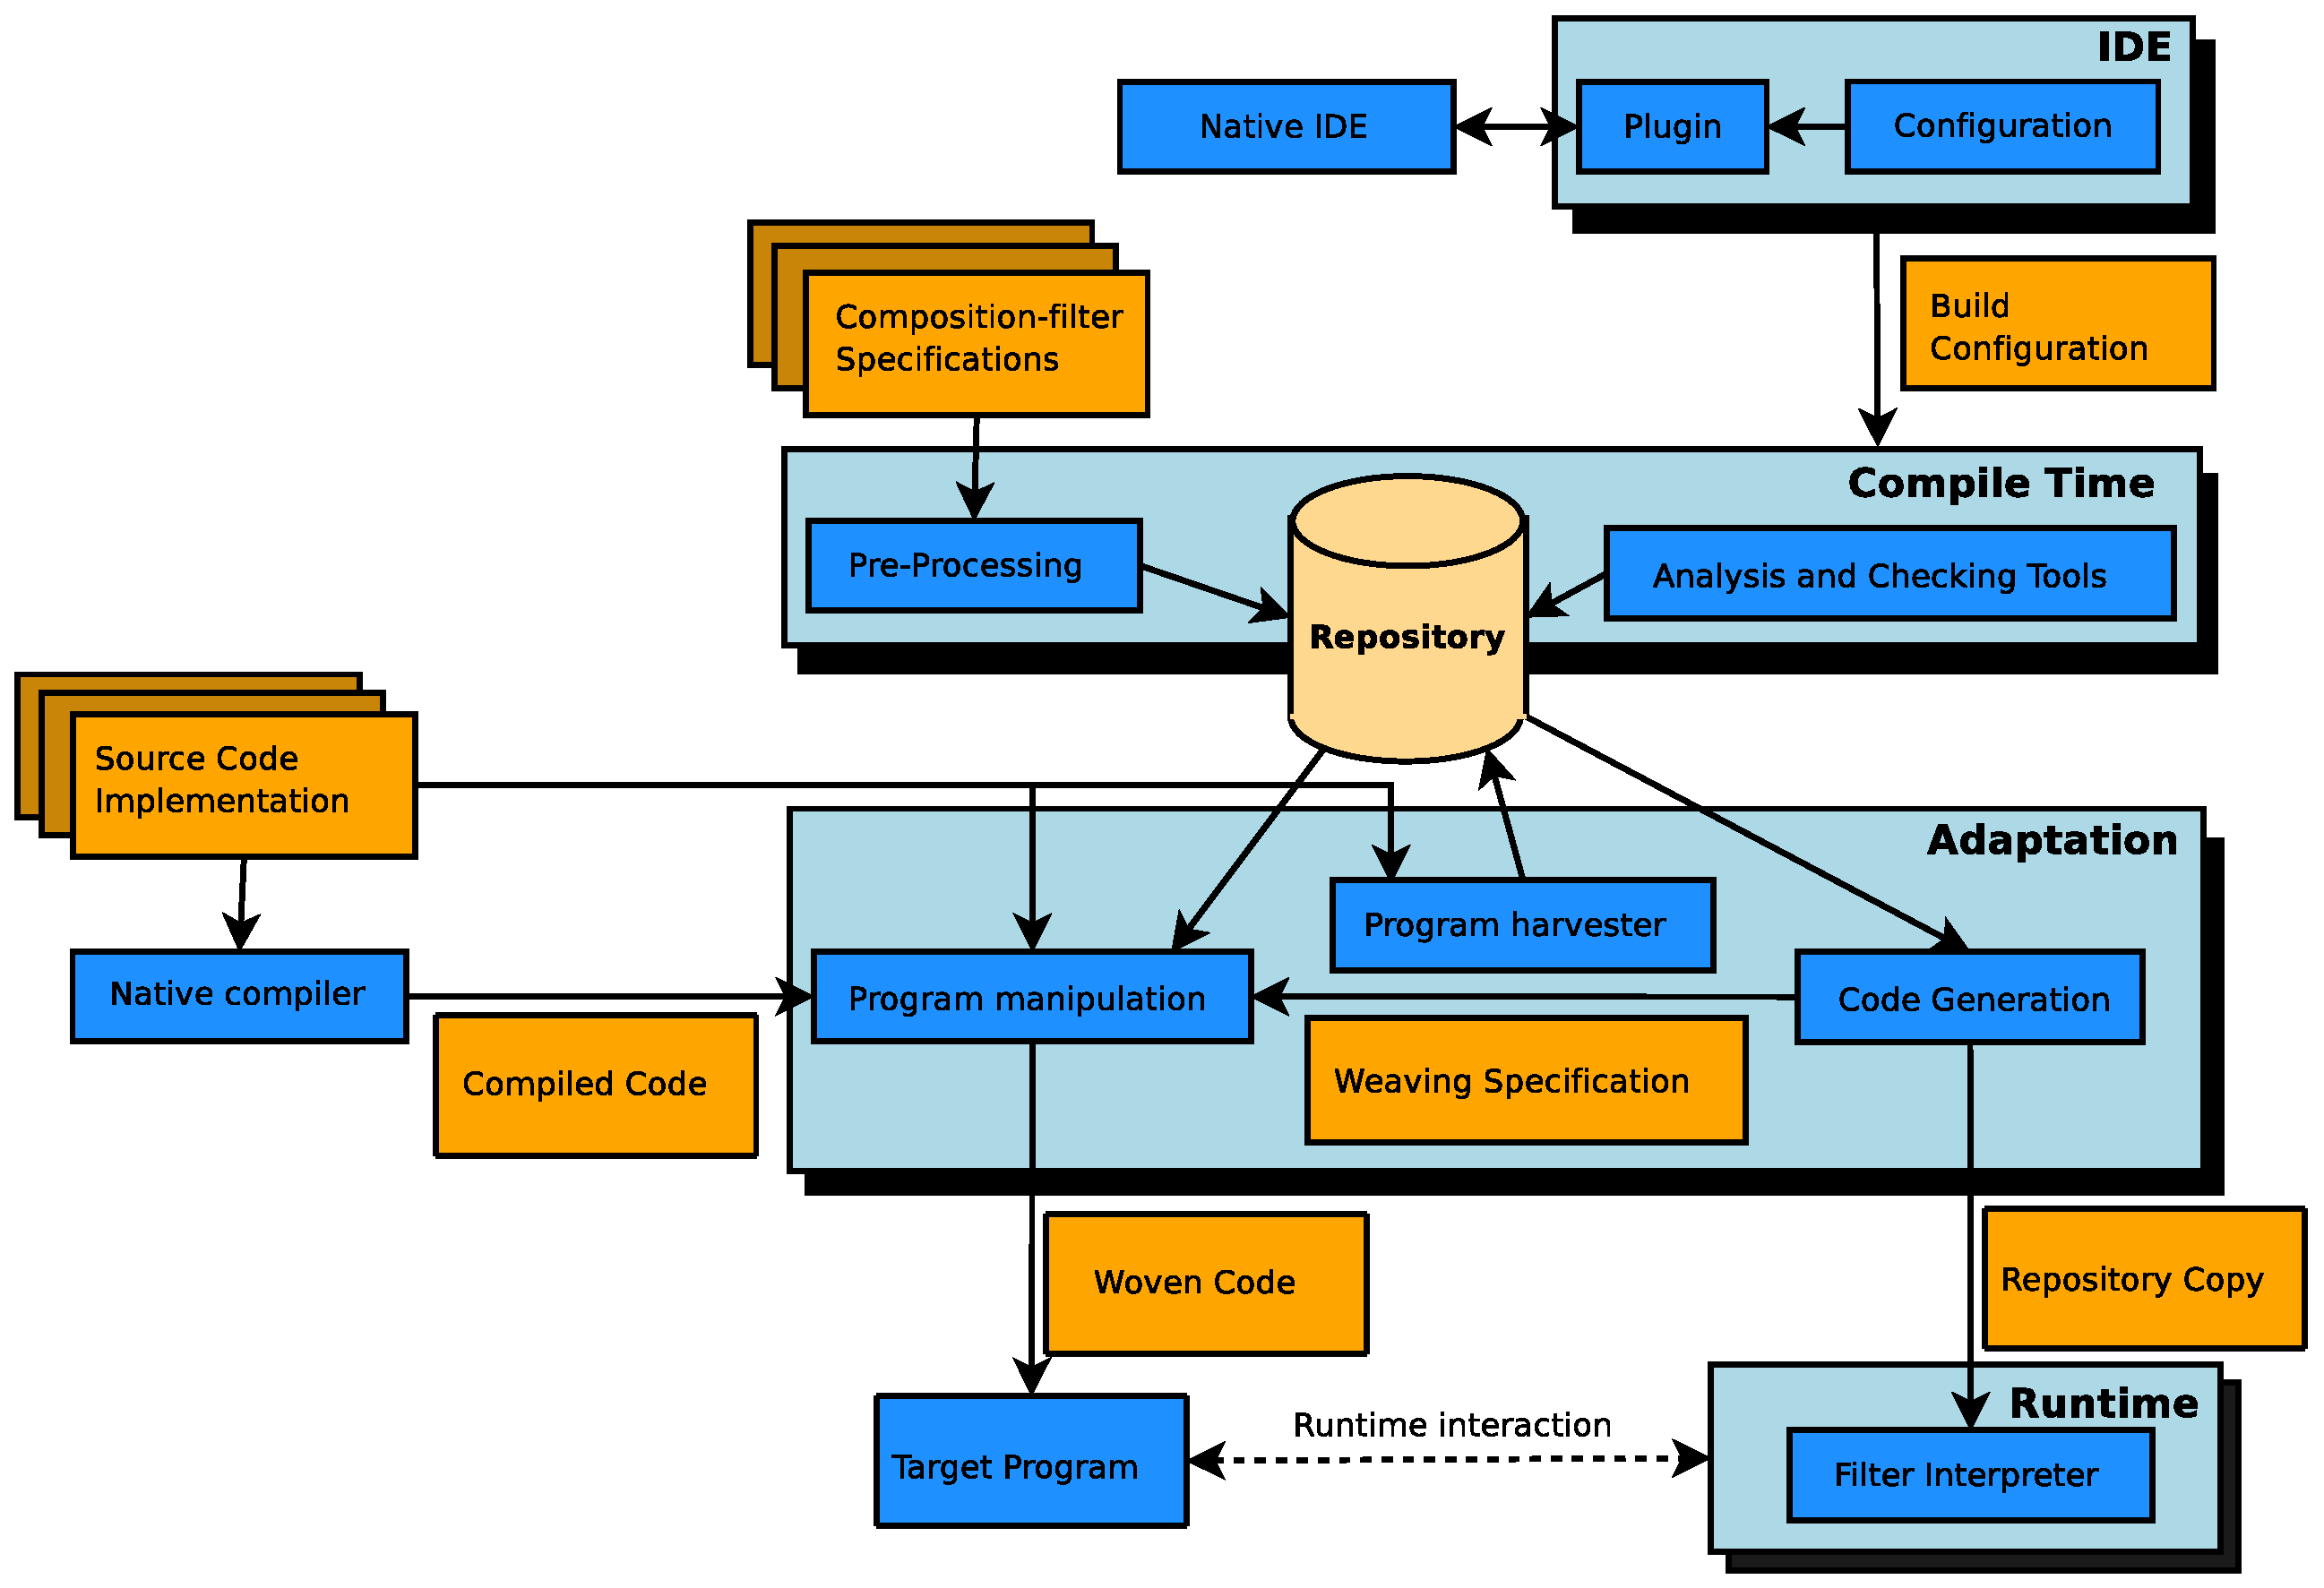
\includegraphics[style=halfheight]{Architecture05}
  \caption[Overview of the \Compose* architecture]{%
    Overview of the \Compose* architecture}
  \label{fig:ComposestarArchitecture}
\end{figure}
An overview of the \Compose* architecture is illustrated in \autoref{fig:ComposestarArchitecture}.
The \Compose* architecture can be divided in four layers~\cite{Nagy2006}: IDE, compile time, adaptation, and runtime. 

\subsection{Integrated Development Environment}
Some of the purposes of the Integrated Development Environment (IDE) layer are to interface with the native IDE and to create a build configuration.
In the build configuration it is specified which source files and settings are required to build a \Compose* application.
After creating the build configuration the compile time is started.

The creation of a build configuration can be done manually or by using a plug-in.
Examples of these plug-ins are the Visual Studio add-in for \Compose*[.NET] and the Eclipse plug-in for \Compose*[J] and \Compose*[C].

\subsection{Compile Time}
The compile time layer is platform independent and reasons about the correctness of the composition filter implementation with respect to the program which allows the target program to be build by the adaptation.

The compile time `pre-processes' the composition filter specifications by parsing the specification, resolving the references, and checking its consistency.
To provide an extensible architecture to facilitate this process a blackboard architecture is chosen.
This means that the compile time uses a general knowledgebase that is called the `repository'.
This knowledgebase contains the structure and metadata of the program which different modules can execute their activities on.
Examples of modules within analysis and validation are the three modules SANE, LOLA and FILTH.
These three modules are responsible for (some) of the analysis and validation of the super imposition and its selectors.

\subsection{Adaptation}
The adaptation layer consists of the program manipulation, harvester, and code generator.
These components connect the platform independent compile time to the target platform.
The harvester is responsible for gathering the structure and the annotations within the source program and adding this information to the knowledgebase.
The code generation generates a reduced copy of the knowledgebase and the weaving specification.
This weaving specification is then used by the weaver contained by the program manipulation to weave in the calls to the runtime into the target program.
The end result of the adaptation the target program which interfaces wit the runtime.

\subsection{Runtime}
The runtime layer is responsible for executing the concern code at the joinpoints.
It is activated at the joinpoints by function calls that are woven in by the weaver.
A reduced copy of the knowledgebase containing the necessary information for filter evaluation and execution is enclosed with the runtime.
When the function is filtered the filter is evaluated.
Depending on if the the condition part evaluates to true, and the matching part matches the accept or reject behavior of the filter is executed.
The runtime also facilitates the debugging of the composition filter implementations.

\section{Platforms}
The composition filters concept of \Compose* can be applied to any programming language, given that certain assumptions are met.
Currently, \Compose* supports three platforms: \dotNET, Java and C\@.
For each platform different tools are used for compilation and weaving.
They all share the same platform independent compile-time.

\Compose*[.NET] targets the \dotNET platform and is the oldest implementation of \Compose*.
Its weaver operates on CIL byte code.
\Compose*[.NET] is programming language independent as long as the programming language can be compiled to CIL code.
An add-in for Visual Studio is provided for ease of development.
\Compose*[J] targets the Java platform and provides a plug-in for integration with Eclipse.
\Compose*[C] contains support for the C programming language.
The implementation is different from the Java and \dotNET counterparts, because it does not have a run-time environment.
The filter logic is woven directly in the source code.
Because the language C is not based on objects, filters are woven on functions based on membership of sets of functions.
Like the Java platform, \Compose*[C] provides a plug-in for Eclipse.

%\section{Features explicit to \Compose*{}}
\section{Features Specific to \Compose*{}}
\label{section:FSTC}
The Composition Filters approach uses a restricted (pattern matching) language to define filters. This language makes it possible to reason about the semantics of the concern. 
\Compose* offers three features that use this possibility, which originate in more control and correctness over an application under construction. These features are:
\begin{description}[style=nextline,noitemsep]
\item [Ordering of filter modules] It is possible to specify how the superimposition of filter modules should be ordered. Ordering constraints can be specified in a fixed, conditional, or partial manner. A fixed ordering can be calculated exactly, whereas a conditional ordering is dependent on the result of filter execution and therefore evaluated at runtime. When there are multiple valid orderings of filtermodules on a join point, partial ordering constraints can be applied to reduce this number. These constraints can be declared in the concern definition;
\item [Filter consistency checking] When superimposition is applied, \Compose* is able to detect if the ordering and conjunction of filters creates a conflict. 
For example, imagine a set of filters where the first filter only evaluates method \emph{m} and another filter only evaluates methods \emph{a} and \emph{b}. 
In this case the latter filter is only reached with method \emph{m}; this is consequently rejected and as a result the superimposition may never be executed. There are different scenarios that lead to these kinds of problems, \eg conditions that exclude each other;
\item [Reason about semantic problems] When multiple pieces of advice are added to the same join point, \Compose* can reason about problems that may occur.
An example of such a conflict is the situation where a real-time filter is followed by a wait filter. Because the wait filter can wait indefinitely, the real-time property imposed by the real-time filter may be violated.
\end{description}
The above mentioned conflict analyzers all work on the assumption that the behavior of every filter is well-defined. This is not the case for the meta filter, its user-undefined, and therefore unpredictable, behavior poses a problem to the analysis tools. 

Furthermore, \Compose* is extended with features that enhance the usability. These features are briefly described below:
\begin{description}[style=nextline,noitemsep]
\item [Integrated Development Environment support] The \Compose* implementations all have a IDE plug-in; \Compose*[.NET] for Visual Studio, \Compose*[J] and \Compose*[C] for Eclipse;
\item [Debugging support] The debugger shows the flow of messages through the filters. It is possible to place breakpoints to view the state of the filters; 
\item [Incremental building process] When a project is build and not all the modules are changed, incremental building saves time.
\end{description}

Some language properties of \Compose* can also be seen as features, being:
\begin{description}[style=nextline,noitemsep]
\item [Language independent concerns] A \Compose* concern can be used for all the \Compose* platforms, because the composition filters approach is language independent;
\item [Reusable concerns] The concerns are easy to reuse, through the dynamic filter modules and the selector language;
\item [Expressive selector language] Program elements of an implementation language can be used to select a set of objects to superimpose on;
\item [Support for annotations] Using the selector, annotations can be woven at program elements. At the moment annotations can be used for superimposition. 
\end{description}



